\documentclass[a4paper,twoside,master.tex]{subfiles}
\begin{document}
\lecture{5}{Wednesday, January 22, 2020}{}
Last lecture, we looked at the case of particles in a box partitioned into two compartments. We wrote down a probabilistic treatment using the binomial distribution, but we can push this forward to gain insight into a function which we can calculate and maximize to find the state of these particles. However we are only halfway there, since that analysis only concerned the positions of the particles and not their momentums.

Today, consider a box separated by a wall which has no hole. However, this wall is diathermal, meaning energy can pass through the wall.


\begin{figure}[h]
    \centering
    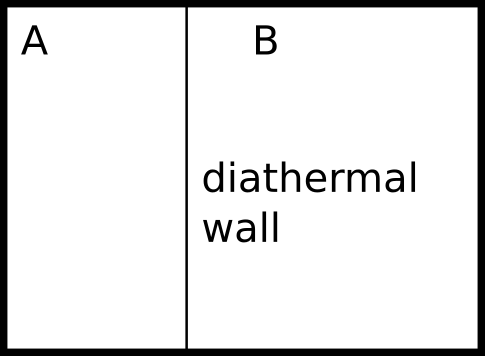
\includegraphics{figures/lec_05_diathermal_box.png}
    \caption{Box with Diathermal Wall}
    \label{fig:box_with_diathermal_wall}
\end{figure}

We consider the energy of each compartment and of the total to be
\begin{equation}
    E_{\alpha} = \sum_{i \in \alpha} \frac{\va{p}^2_{\alpha,i}}{2m}
\end{equation}

There are many microstates which we can define (a single microstate is a set of momenta $ \{\va{p}_1,\va{ p}_2, \cdots,\va{ p}_N\} $), but only certain ones will satisfy the constraint $ E = \sum_i \frac{\va{p}^2_i}{2m} $.

These microstates live on a $ 3N-1 $-dimensional hyperspace. Consider that all microstates are equally likely. This means
\begin{equation}
    \Pr(\{\va{p}\}) = \frac{\delta(E - \sum_i \frac{\va{p}^2_i}{2m})}{\int \dd[3N]{p} \delta(E - \sum_i \frac{\va{p}_i^2}{2m})}
\end{equation}

This is the original sin of stat mech: we will not derive this equation, but take it for granted. It does seem reasonable, since it picks out allowed microstates and is obviously normalized.

What is the probability of getting a value $ E_A $? We can use the transformation theorem:
\begin{align}
    \Pr_{A}(E_A) &= \int \dd[3N]{p} \Pr(\{\va{p}\}) \delta\left(E_A - \sum_{i \in A} \frac{\va{p}^2_i}{2m}\right) \\
    &= \frac{\int \dd[3N]{p} \delta\left( E - \sum_j \frac{\va{p}_j^2}{2m} \right) \delta\left( E_A - \sum_{i \in A} \frac{\va{p}_i^2}{2m} \right)}{\int \dd[3N]{p} \delta\left( E - \sum_j \frac{\va{p}_j^2}{2m} \right)} \\
    &= \frac{\int \dd{p_A} \delta\left( E_A - \sum_{i \in A} \frac{\va{p}_i^2}{2m} \right) \int \dd{p_B} \delta\left( \overbrace{E - \sum_{j \in A} \frac{\va{p}^2_j}{2m}}^{E_B} - \sum_{j \in B} \frac{\va{p}^2_j}{2m} \right)}{\int \dd{p} \delta\left( E - \sum_j \frac{\va{p}_j^2}{2m} \right)} \\
    &= \frac{\int \dd{p_A} \delta\left( E_A - \sum_{i \in A} \frac{\va{p}_i^2}{2m} \right) \int \dd{p_B} \delta\left( E_B - \sum_{i \in B} \frac{\va{p}_i^2}{2m} \right)}{\int \dd{p} \delta\left( E - \sum_i \frac{\va{p}^2_i}{2m} \right)}
\end{align}
This final equation is Equation $ 6.3 $ in the book, and is just given as obvious (while it clearly isn't).

These integrals all have the same basic form. Let's call them functions:
\begin{equation}
    \Pr_{A}(E_A) = \frac{\Omega_E(E_A, N_A) \vdot \Omega_E(E_B, N_B)}{\Omega_E(E, N)}
\end{equation}
where
\begin{equation}
    \Omega_E(E, N) = \int \dd{p} \delta\left( E - \sum_i \frac{\va{p}_i^2}{2m} \right)
\end{equation}

The structure is now precisely the same as our previous work with position, although this integral is not exactly as simple as the summation we had before. Let's expand this integral so we can understand what's going on:

\begin{equation}
    \Omega_E(E, N) = \int \dd[3]{p_1} \dd[3]{p_2} \cdots \dd[3]{p_N} \delta\left( E - \frac{1}{2m} \sum_i\va{ p}_i^2 \right)
\end{equation}
This is an integral over a $ 3N $-dimensional space. Fortunately, the function we are integrating is not terrible, since the variable we are integrating over enters in the form
\begin{equation}
    \sum_i\va{ p}_i^2
\end{equation}
which is just the squared distance from the origin of the momentum vector. If we were in three dimensions, this would be a spherically symmetric problem, since $ x^2 + y^2 + z^2 = r^2 $, and we would be tempted to go into spherical coordinates and just integrate over $ r $. In three dimensions, we take $ \dd[3]{p} \to \dd{p} 4 \pi p^2 $. We have to extend this to $ N $-dimensions. For now, let's write this differential as
\begin{equation}
    \dd[3]{p_1} \dd[3]{p_2} \cdots \dd[3]{p_N} \to \dd{p} p^{3N - 1} S_{3N}
\end{equation}
where $ S_{3N} $ is the surface area of a unit sphere in $ \R^{3N} $ (such that $ S_3 = 4 \pi $).

Now our $ \Omega_E $ function looks like:
\begin{align}
    \Omega_E(E, N) &= \int_{0}^{\infty} \dd{p} p^{3N-1} S_{3N} \delta(E - \frac{1}{2m} p^2) \\
    &= \int_0^{\infty} \dd{p} p p^{3N-2} S_{3N} \delta\left( E - \frac{p^2}{2m} \right)
\end{align}
Let's now make the substitution
\begin{equation}
    x = \frac{p^2}{2m} \to p = \sqrt{2mx} \quad \dd{x} = \frac{p \dd{p}}{m} \to m \dd{x} = p \dd{p}
\end{equation}
so
\begin{equation}
    \Omega_E(E,N) = \int_0^{\infty} \dd{x} m (2mx)^{\frac{3N-2}{2}} S_{3N} \delta(E-x) = m S_{3N}(2mE)^{\frac{3N-2}{2}}
\end{equation}

Notice we already have the energy dependence\textemdash the $ S_{3N} $ term is just an $ N $-dependent scale factor. However, it would be nice to know what it actually is before we compute the final probability.

What is the surface area of a sphere in $ M $-dimensional space?
\begin{equation}
    \int \dd{x} e^{-x^2} = \pi^{\frac{1}{2}}
\end{equation}
Now we will take this integral and raise it to the power of $ M $:
\begin{align}
    \pi^{\frac{M}{2}} = \left[ \int \dd{x} e^{-x^2} \right]^M \\
    &= \int \dd{x_1} \dd{x_2} \cdots \dd{x_M} e^{-(x_1^2 + x_2^2 + \cdots + x_M^2)} \\
    \text{Use spherical coordinates: } &= \int_0^{\infty} \dd{x} x^{M-1} S_M e^{-x^2}
\end{align}
Now use the substitution
\begin{equation}
    t = x^2 \to x = \sqrt{t} \quad \dd{x} = \frac{1}{2 \sqrt{t}} \dd{t}
\end{equation}
\begin{align}
    \pi^{\frac{M}{2}} &= \int_0^{\infty} \frac{\dd{t}}{2 \sqrt{t}} t^{\frac{M-1}{2}} S_M e^{-t} \\
    &= \frac{1}{2} S_M \int_0^{\infty} \dd{t} t^{\frac{M}{2} - 1} e^{-t} \\
    &= \frac{1}{2} S_M \Gamma\left( \frac{M}{2} \right)
\end{align}

The gamma function has the property that
\begin{equation}
    \Gamma(N+1) = N! \qfor N \in \mathbb{N}
\end{equation}
We can finally write our equation for $ S_M $:
\begin{equation}
    S_M = \frac{2 \pi^{\frac{M}{2}}}{\Gamma\left( \frac{M}{2} \right)} = \frac{2 \pi^{\frac{M}{2}}}{\left( \frac{M}{2} - 1 \right)!} = \frac{M \pi^{\frac{M}{2}}}{\left( \frac{M}{2} \right)!}
\end{equation}
so we can finally write down

\begin{equation}
    \Omega_E(E, N) = \frac{3N \pi^{\frac{3N}{2}}}{\left( \frac{3N}{2} \right)!} m(2mE)^{\frac{3N-2}{2}}
\end{equation}



\end{document}
